\documentclass{ximera}

\newcommand{\RR}{\mathbb R}
\renewcommand{\d}{\,d}
\newcommand{\dd}[2][]{\frac{d #1}{d #2}}
\renewcommand{\l}{\ell}
\newcommand{\ddx}{\frac{d}{dx}}
\newcommand{\dfn}{\textbf}
\newcommand{\eval}[1]{\bigg[ #1 \bigg]}


\title[Dig-In:]{A tale of three integrals}

\begin{document}
\begin{abstract}
  At this point we have three ``different'' integrals. 
\end{abstract}
\maketitle

At this point we have three different ``integrals.'' Let's see if we
can sort out the differences.

\section{Indefinite integrals}

Indefinite integrals, also called \dfn{antiderivatives} compute
classes of functions:
\[
\int f(x) \d x = \text{``a class of functions whose derivative is $f$''}
\]
Here there are no limits of integration, and your answer will have a
``$+C$'' at the end. Pay attention to the notation:
\begin{center}
  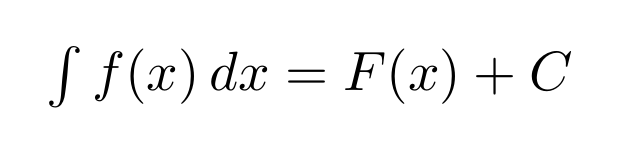
\begin{tikzpicture}[scale=2,every node/.style={transform shape}]
    \node at (0,0) {
      $\int f(x) \d x = F(x) + C$
      };
  \end{tikzpicture}
\end{center}
Where $F'(x) = f(x)$.
\begin{explanation}%%%BADBAD I would like no environment here.
  Indefinite integrals
  \wordChoice{\choice{have}\choice[correct]{do not have}} limits of
  integration, and they compute \wordChoice{\choice{signed
      area}\choice{an antiderivative of $f$}\choice[correct]{a class
      of antiderivatives for $f$}}.
\end{explanation}


\section{Accumulation functions}

Accumulation functions, also called \dfn{area functions} compute accumuated area:
\[
\int_a^x f(t) \d t = \text{``a function $F$ whose derivative is $f$''}
\]
This is a function of $x$ whose derivative is $f$, with the additional
property that $F(a)=0$.  Pay attention to the notation:
\begin{center}
  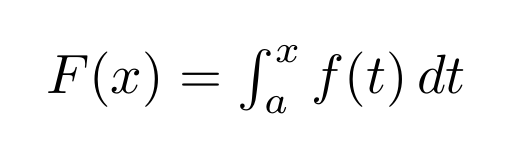
\begin{tikzpicture}[scale=2,every node/.style={transform shape}]
    \node at (0,0) {
      $F(x)=\int_a^x f(t) \d t$
      };
  \end{tikzpicture}
\end{center}
Where $F'(x) = f(x)$.
\begin{explanation}%%%BADBAD I would like no environment here.
  Accumulation functions \wordChoice{\choice[correct]{have}\choice{do
      not have}} limits of integration, and they compute
  \wordChoice{\choice{signed area}\choice[correct]{an antiderivative of
      $f$}\choice{a class of antiderivatives for $f$}}.
\end{explanation}

\section{Definite integrals}

Definite integrals compute signed area:
\[
\int_a^b f(x) \d x = \text{``the signed area between the $x$-axis and $f$''}
\]
Here we always have limits of integration, both of which are
numbers. Moreover, definite integrals have definite values, the signed
area between $f$ and the $x$-axis. Pay attention to the notation:
\begin{center}
  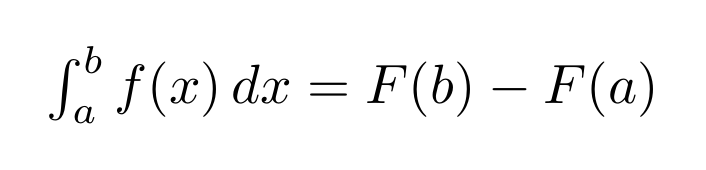
\begin{tikzpicture}[scale=2,every node/.style={transform shape}]
    \node at (0,0) {
      $\int_a^b f(x) \d x = F(b)-F(a)$
      };
  \end{tikzpicture}
\end{center}
Where $F'(x) = f(x)$.
\begin{explanation}%%%BADBAD I would like no environment here.
  Definite integrals \wordChoice{\choice[correct]{have}\choice{do
      not have}} limits of integration, and they compute
  \wordChoice{\choice[correct]{signed area}\choice{an antiderivative of
      $f$}\choice{a class of antiderivatives for $f$}}.
\end{explanation}

\end{document}
